%
% File acl2017.tex
%
%% Based on the style files for ACL-2015, with some improvements
%%  taken from the NAACL-2016 style
%% Based on the style files for ACL-2014, which were, in turn,
%% based on ACL-2013, ACL-2012, ACL-2011, ACL-2010, ACL-IJCNLP-2009,
%% EACL-2009, IJCNLP-2008...
%% Based on the style files for EACL 2006 by
%%e.agirre@ehu.es or Sergi.Balari@uab.es
%% and that of ACL 08 by Joakim Nivre and Noah Smith

\documentclass[12pt,a4paper]{article}
\usepackage[hyperref]{acl2017}
\usepackage{times}
\usepackage{latexsym}
\usepackage{amsmath}
\usepackage{url}
\usepackage{graphicx}
\usepackage{amssymb}
\usepackage[noend]{algpseudocode}
\usepackage{algorithmicx,algorithm}

\aclfinalcopy % Uncomment this line for the final submission
%\def\aclpaperid{***} %  Enter the acl Paper ID here

%\setlength\titlebox{5cm}
% You can expand the titlebox if you need extra space
% to show all the authors. Please do not make the titlebox
% smaller than 5cm (the original size); we will check this
% in the camera-ready version and ask you to change it back.

\newcommand\BibTeX{B{\sc ib}\TeX}

\title{Final Project: Smart Gomoku Agent}

\author{Tianxiao Hu \\
  School of Computer Science\\
  Fudan University\\
  {\tt txhu14@fudan.edu.cn} \\\And
  Hui Xu \\
  School of Data Science\\
  Fudan University\\
  {\tt xuhui14@fudan.edu.cn} \\\And
  Bing Zhang \\
  School of Data Science\\
  Fudan University\\
  {\tt 14307130338@fudan.edu.cn}
}

\date{\today}

\begin{document}
\maketitle
\begin{abstract}
Our Gomoku game support two types of games, including HUMAN VS AI and AI VS AI. A well-designed user interface is provided. 3 versions of AI algorithms are implemented: \textbf{Greedy}, \textbf{Minimax Search} and \textbf{Monte Carlo Tree Search}. We use Github\footnote{https://github.com/TianxiaoHu/GomokuAgent} to manage our codes.

% TODO
\end{abstract}

\section{Introduction}
Gomoku, also called ``five in a row'', is a board game which originates from Japan. It is a game played on a Go board typically of size 15 x 15. In the game, players will take turns placing stones until a player has managed to connect 5 in a row.

\begin{figure}[!ht]
\centering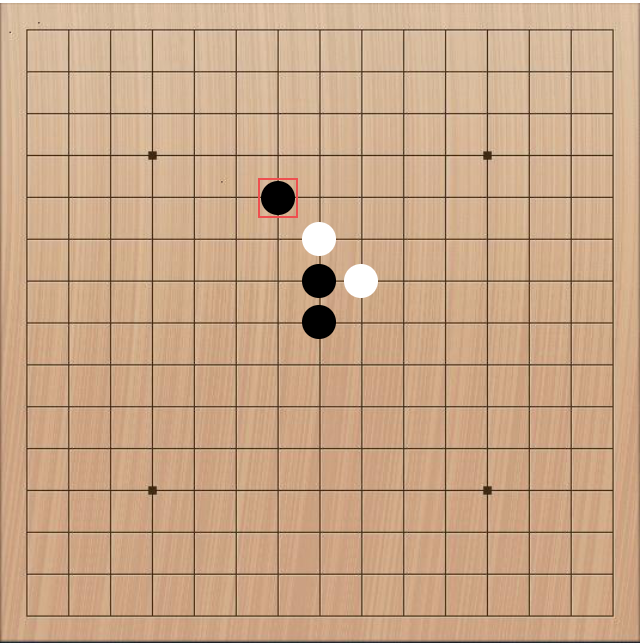
\includegraphics[width=3in]{2.png}
\caption{A Typical Gomoku Game}
\end{figure} 

This project is aimed to develop a smart agent for Gomoku game. We use 3 main strategies to implement the agent: \textbf{Greedy}, \textbf{Minimax Search} and \textbf{Monte Carlo Tree Search(MCTS)}. We will introduce them in details in the following sections.\\
We also developed a user interface for Gomoku game. Special thanks to open source project gobang\footnote{https://github.com/lihongxun945/gobang} for the beautiful design of the web page! HUMAN VS AI and AI VS AI are both supported. 

\section{Evaluation Function}
First of all, in order to quantify the properties of the current situation, we construct an evaluation function to estimate the win-probability. And naturally, the evaluation function will incorporate a great deal of the knowledge about the Gomoku game. Therefore, the evaluation can be either naive or complicated, which depends on the your understanding towards the Gomoku game. In general, the more complex the evaluation is, the slower the program will get over time.

In this section, we mainly propose two versions of the evaluation function.

\subsection{The First Version}
The general idea of the first version is fairly simple. As is known to all, the object of the game is to be the first player to achieve five pieces in a row, horizontally, vertically or diagonally. Therefore, we can focus only on the five continuous positions on the chess-board, hereinafter called ``five-tuple''. Generally, the chess-board is $15\times 15$, having 572 five-tuples in all. Then we can assign a score to every five-tuple based on the number of the black and white pieces in it. Here we ignore the relative position of pieces. Then the evaluation to a given situation is the sum of the score of all 572 five-tuples. Suppose we take piece "x" and opponent takes piece "o", then the score table for me is displayed as follow,
\begin{table}[h]
\centering
\begin{tabular}{c|c}
\hline
Five-Tuple&Score \\
\hline
x&15\\
xx&400\\
xxx&1800\\
xxxx&100000\\
xxxxx&10000000\\
o&-35\\
oo&-800\\
ooo&-15000\\
oooo&-800000\\
ooooo&-10000000\\
Blank&7\\
Polluted&0\\
\hline
\end{tabular}
\end{table}

\noindent\begin{small}\emph{Note the score to blank five-tuple is 7 rather than 0. This is because there is worse condition, where the five-tuple is polluted, i.e., both black and white pieces in the tuple.}\end{small}

The first version of the evaluation function is fairly simple and works rapidly. Nevertheless, after trying dozens of man-machine games, we find the agent can make some stupid mistakes, which result from its excessively simple evaluation function. Actually, the defect can be well solved by applying Minimax algorithm, but at a high price of the computing resource.
\subsection{The Second Version}
Then we intend to add more knowledge to the evaluation function to make it ``smarter''.

In the second version of the evaluation function, we take more account of chess-types, or in other words, the relative position of the pieces.

For every non-blank position on the chess-board, we take it as the center and extend four positions to both sides horizontally, vertically and diagonally. Then we can obtain four nine-tuples. For each nine-tuple, we check its chess-type and assign a score according to the new score table. Add up these four scores and we can get the score of this position.

Finally, our score is the sum of all positions occupied by our pieces while the opponent's score is the sum of all positions occupied by his pieces. And the evaluation to current situation is the difference of our score and opponent's score.

The new score table is stated below,
\begin{table}[h]
\centering
\begin{tabular}{c|c|c}
\hline
Chess-Type&Self-Score&Opponent-Score  \\
\hline
Five&1000000&1000000\\
Alive-Four&20000&100000\\
CoDash-Four&6100&65000\\
GapDash-Four&6000&65000\\
CoAlive-Three&1100&5500\\
GapAlive-Three&1000&5000\\
Asleep-Three&300&200\\
Alive-Two&100&90\\
Asleep-Two&10&9\\
One&3&4\\
\hline
\end{tabular}
\end{table}

\noindent\begin{small}\emph{Note the names of the chess-types are fabricated by ourselves because we can't find accurate translation to these terms. If you are interest in the exact chess mode corresponding to the chess-types, please refer to the code or contact us.}\end{small}

\subsection{Using Genetic Algorithm to find Better Evaluation Function}
You may find in the score table, the chess-types and corresponding self-scores and opponent scores are quite subjective. Thus, we applied genetic algorithm to find a better evaluation function, which is inspired by the process of natural selection. 

We initialize the algorithm by setting the original score table as the very first generation. Afterwards, it can breed a new generation by randomly plus or minus 3\% specific chess-type score. The parent agent will play with each child agent 100 times and find the best children as the new parent. When the new generation can't defeat their parent, the algorithm comes to an end.

The results are as follow:
% new score~~
\begin{table}[h]
\centering
\begin{tabular}{c|c|c}
\hline
Chess-Type&Self-Score&Opponent-Score  \\
\hline
Five&1000000&1000000\\
Alive-Four&20000&100000\\
CoDash-Four&6100&65000\\
GapDash-Four&6000&65000\\
CoAlive-Three&1100&5500\\
GapAlive-Three&1000&5000\\
Asleep-Three&300&200\\
Alive-Two&100&90\\
Asleep-Two&10&9\\
One&3&4\\
\hline
\end{tabular}
\end{table}


\section{Greedy Algorithm}
Greedy algorithm is an algorithmic paradigm that follows the problem solving heuristic of making the locally optimal choice at each stage, with the hope of finding a global optimum.

For our Gomoku agent, the evaluation function is exactly the so-called problem solving heuristic.
And the implementation of the greedy search is elaborated as follows:
\begin{algorithm}[h]
\caption{Greedy Search}
\hspace*{0.02in} {\bf Input:} 
chess board\\
\hspace*{0.02in} {\bf Output:} 
position of move
\begin{algorithmic}
\For{each position (i, j) on the board}
  \If{position (i, j) is blank}
    \State suppose place my stone on (i, j)
		\State calculate my score: myScore
        		\State calculate opponent score: opScore
        		\State score(i, j) = myScore - opScore
	\EndIf
\EndFor
\Return the position with the maximum score
\end{algorithmic}
\end{algorithm}

%\LinesNumbered
%\KwIn{chess board}
%\KwOut{position of move}
%
%\For{each position (i,j) on the board}{
%  \If{position (i,j) is blank}{
%    suppose place my stone on (i,j)\;
%        calculate my score: myScore\;
%        calculate opponent score: opScore\;
%        score(i,j) = myScore - opScore;
%  }
%
%}
%Return the position with the maximum score
%\end{algorithm}

However, after dozens of games, we find the greedy strategy does not in general produce an optimal solution. On the one hand, owing to the limitation of the evaluation function, the evaluated score of the current situation can't describe the win-probability precisely. On the other hand, this is also the inherent defect of the greedy algorithm. But nonetheless a greedy heuristic may yield locally optimal solutions that approximate a global optimal solution in a reasonable time, which is appealing when solving many other problems.


\section{Learn Openings from Game Record}
After testing our agents for a number of games, we found opening is fairly important for Gomoku. If our agent is playing with a experienced human, it will easily lose the advantage during the opening. However, there are hundreds of different openings and they are hard to compute or collect. To solve the problem, we let our agent learn from 5581 top-level game records\footnote{http://game.onegreen.net/Soft/HTML/47233.html}. If current game matches some sequences of initial moves in the game records, it will compute scores for records and find the next step having the highest score.

\section{Minimax Algorithm}

\subsection{Introduction to Minimax and Alpha-Beta Prunning}

In general games, the maximin value of a player is the largest value that the player can be sure to get without knowing the actions of the other players; equivalently, it is the smallest value the other players can force the player to receive when they know his action.\\
Calculating the maximin value of a player is done in a worst-case approach: for each possible action of the player, we check all possible actions of the other players and determine the worst possible combination of actions - the one that gives player $i$ the smallest value. Then, we determine which action player $i$ can take in order to make sure that this smallest value is the largest possible.

\begin{figure}[!h]
\centering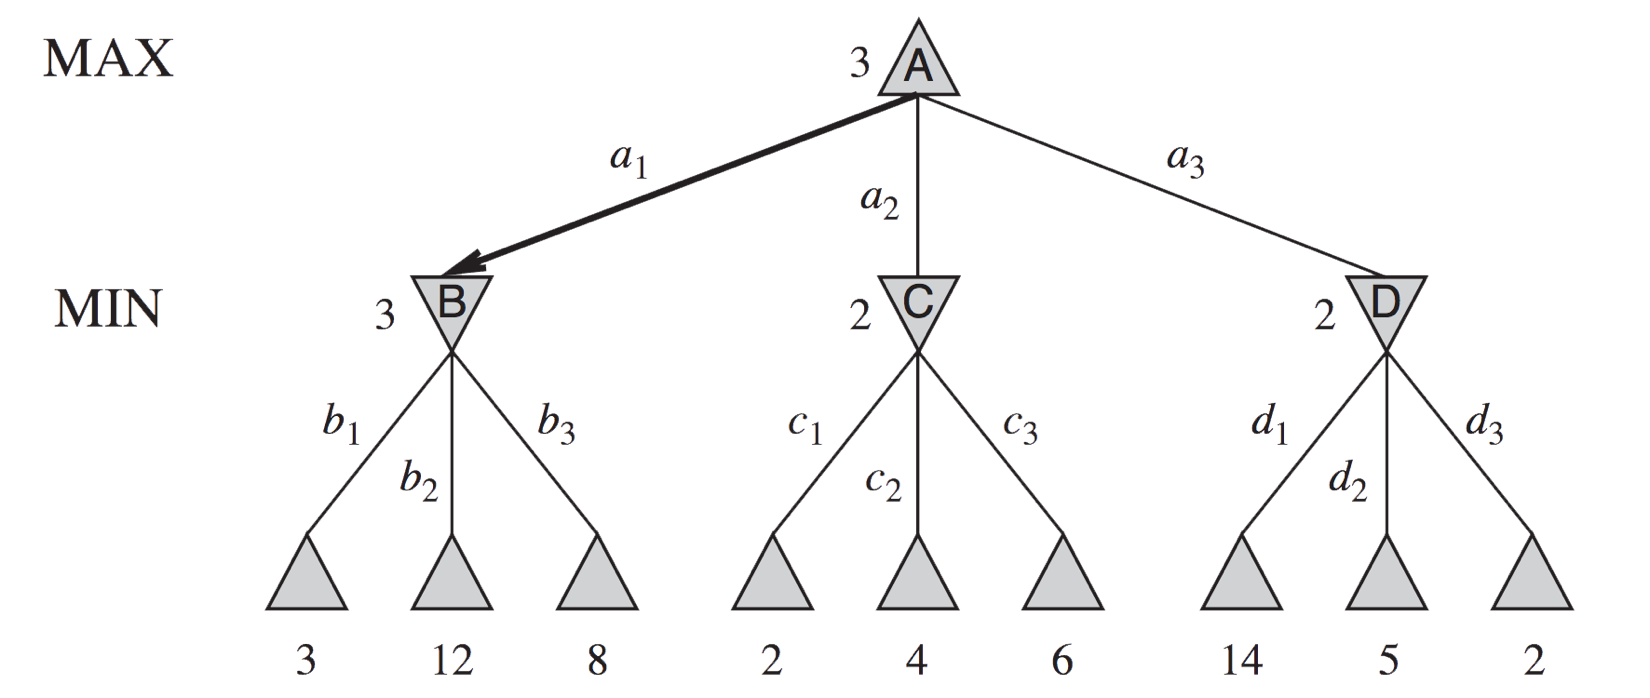
\includegraphics[width=3in]{3.png}
\caption{Example: Minimax Search}
\end{figure} 

In Gomoku game, we use \textbf{evaluation function} to score each board. After a player has placed a stone on the board, a new state is created right after the old. Afterwards, agents can search the tree and return the best choice. However, due to the large search space of Gomoku, the tree will expand rapidly and lead to a unbearable waiting time. We employed Alpha-Beta Prunning to accelerate our agent.

Alpha–Beta pruning is a search algorithm that seeks to decrease the number of nodes that are evaluated by the Minimax algorithm in its search tree. It stops completely evaluating a move when at least one possibility has been found that proves the move to be worse than a previously examined move. Such moves need not be evaluated further. 

\begin{figure}[!h]
\centering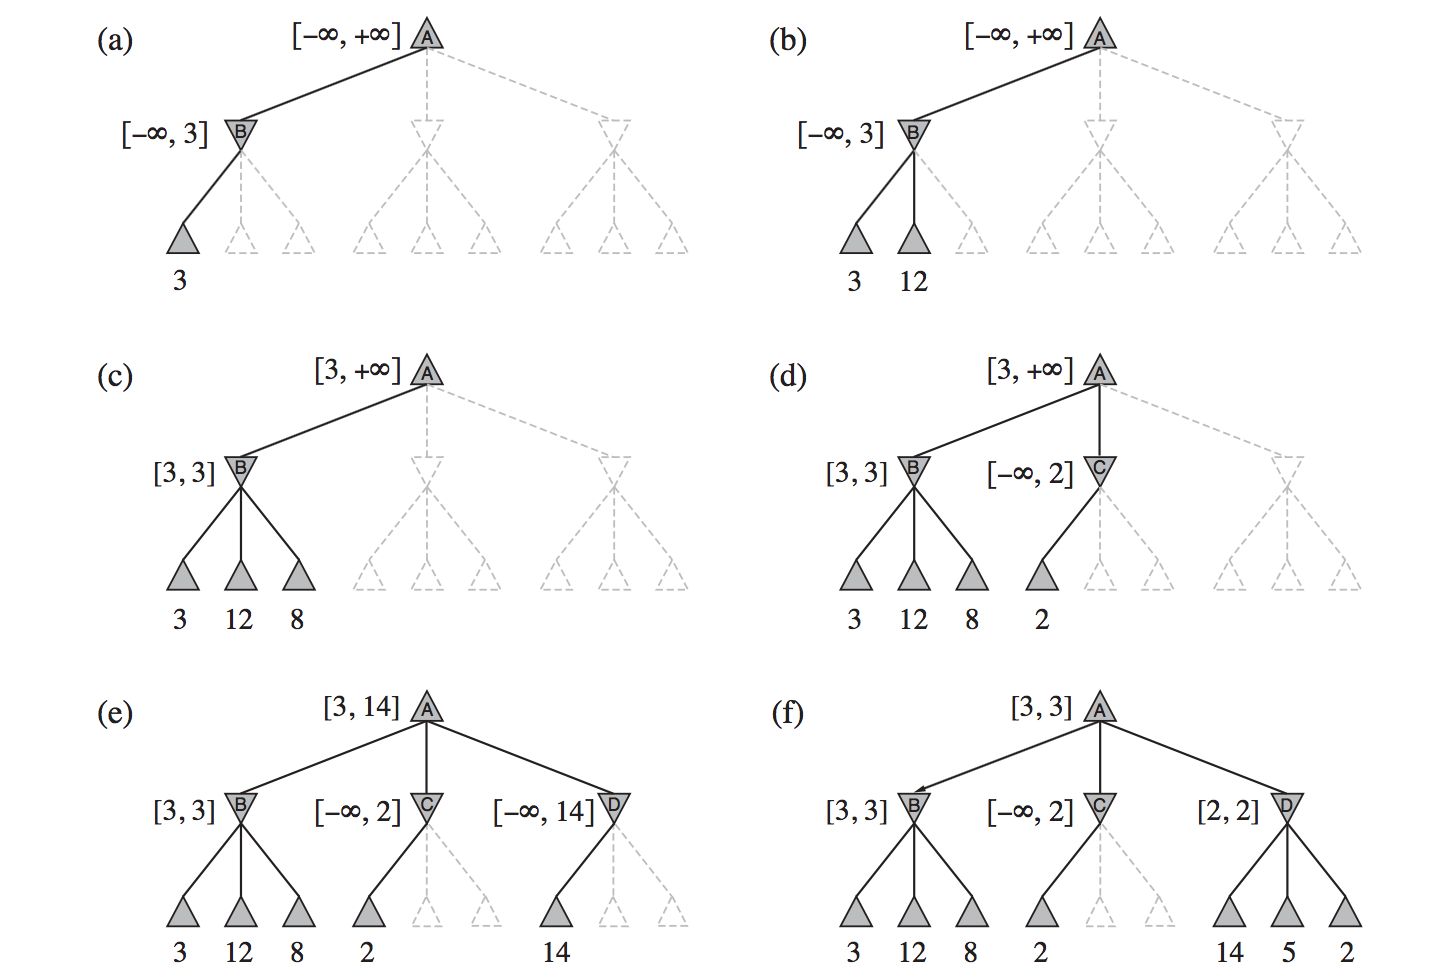
\includegraphics[width=3in]{4.png}
\caption{Example: Minimax Search}
\end{figure}

Our pseudocode is listed below.

\begin{algorithm}[!h]
\caption{Alpha-Beta Pruning algirithm} 
\hspace*{0.02in} {\bf function} 
alphabeta(node, depth, $\alpha, \beta$, maximizingPlayer)
\begin{algorithmic}
\If{depth = 0 or node is a terminal node}
	\State \Return the heuristic value of node
	\If{maxmizingPlayer}
		\State v $\gets - \infty$ 
		\For{each child of node}
			\State v $\gets max(v, alphabeta(child, depth - 1, \alpha, \beta, FALSE)$
			\State $\alpha \gets max(\alpha, v)$ 
			\If{$\beta \leq \alpha$}
				\State break
			\EndIf
		\State \Return v
		\EndFor
	\Else
		\State $v \gets + \infty$
		\For{each child of node}
			\State v $\gets min(v, alphabeta(child, depth - 1, \alpha, \beta, TRUE)$
			\State $\beta \gets max(\beta, v)$ 
			\If{$\beta \leq \alpha$}
				\State break
			\EndIf
		\State \Return v
		\EndFor
	\EndIf
\EndIf
\end{algorithmic}
\end{algorithm}


\subsection{Speed Optimization}
The depth of search tree is an important parameter in Minimax Search. If layers searched not enough, our agent will be really short-sighted. However, for the sake of Python's efficiency, our naive implementation can only search for 2 layers in 1 second. If we force it to search 4 layers, the waiting time will become 10 seconds. Further optimization is needed.

\begin{itemize}
\item \textbf{Less Search States}\\
We explore less search state for each player. Instead of search all possible place for a stone, we only consider places near stones which are already placed in the board. 
\item \textbf{Zobrist Hashing States in Memory}\\
During the expanding of the search tree, some nodes may share the same state. Their scores will be the same so we need not calculate them twice. We save each state and its score in memory to accelerate the agent.\\
However, a state is hard to perform hashing. We use Zobrist Hashing to represent states. Zobrist Hashing starts by randomly generating bitstrings for each possible element of a board game, i.e. for each combination of a piece and a position. Now any board configuration can be broken up into independent position components, which are mapped to the random bitstrings generated earlier. The final Zobrist Hashing is computed by combining those bitstrings using bitwise XOR. When updating positions, rather than computing the hash for the entire board every time, the hash value of a board can be updated simply by XOR out the bitstring for positions that have changed, and XOR in the bitstrings for the new positions.  
\item \textbf{Python's Numba Package}\\
Our implementation is based on Python's scientific computing packages Numpy. We use Numba package to accelerate it. Numba is an Open Source NumPy-aware optimizing compiler for Python. It uses the LLVM compiler infrastructure to compile Python to machine code. This optimized function runs 200 times faster than the interpreted original function on a long NumPy array; and it is 30\% faster than NumPy's builtin \emph{sum()} function\footnote{https://en.wikipedia.org/wiki/Numba}.

\end{itemize}

Our optimized Alpha-Beta Prunning can search 8 layers in 1 second. And it turned out to be really hard to defeat especially when it's on the offensive.

\section{Monte Carlo Tree Search}
\subsection{Introduction to MCTS and UCT}
\par Monte Carlo Tree Search (MCTS) is a tree search technique expanding the search tree based on random sampling of the search space. The application of Monte Carlo tree search in games is based on many playouts. In each playout, the game is played out to the very end by selecting moves at random. The final game result of each playout is then used to weight the nodes in the game tree so that better nodes are more likely to be chosen in future playouts. The strategy is going to have to balance playing all of the machines to gather that information, with concentrating the plays on the observed best machine. One strategy, called UCB1, does this by constructing statistical confidence intervals for each machine.

\begin{figure*}[!ht]
\centering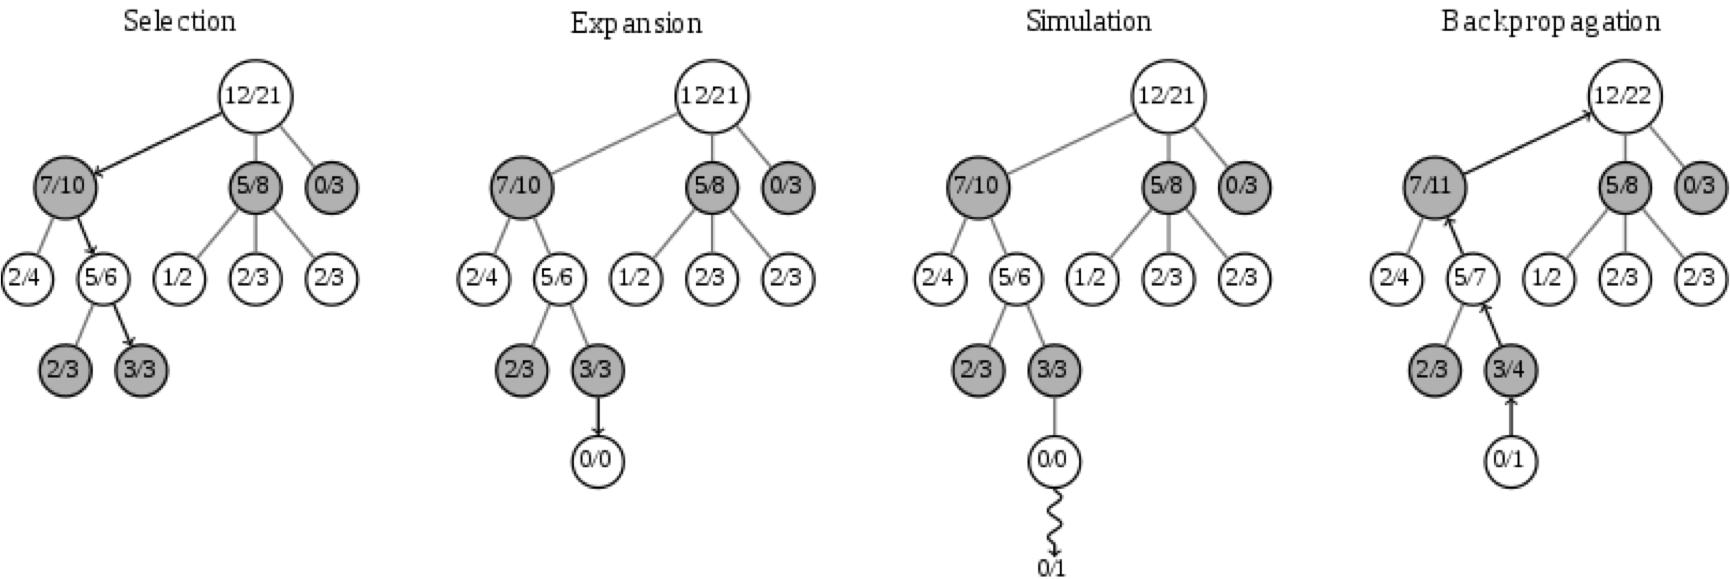
\includegraphics[width=6in]{1.png}
\caption{Example: Monte Carlo Tree Search}
\end{figure*}

\begin{displaymath}
\bar{x}_i \pm \sqrt{\frac{C\ln n}{n_i}}
\end{displaymath}
\begin{center}
$\bar{x}_i$: the mean playout for machine \emph{i}\\
$n_i$: the number of plays of machine \emph{i} \\
$n$: the total number of plays
\end{center}
Then, the strategy is to pick the machine with the highest upper bound each time. Upper Confidence bound applied to Trees (UCT)
is MCTS with UCB strategy.
\par For Gomoku game, MCTS starts with a chess board and walk chess randomly until the end. The process is repeated many times which eliminates the best move for the current chess board. Each round of Monte Carlo tree search consists of four steps:

\begin{itemize}
\item Selection:
Build the root node based on the current chess board and generate all of its child nodes. The move to use would be chosen by the UCB1 algorithm and applied to obtain the next position to be considered. 
\item Expansion:
Selection would then proceed until reach a position where not all of the child positions have statistics recorded. 
\item Simulation:
If the node hasn't been simulated, then do a typical Monte Carlo simulation for chess game. Else, generate a random child node for the leaf node and do the simulation.
\item Backpropagation:
Update the reward of the simulation (generally 0 for lose and 1 for win) to the leaf node and its ancestor node. Meanwhile add the number of view for every node in the search path.
\end{itemize}
\par Repeat the playouts for many times until reach the search time or max search times and we can get the best move by selecting the maximum reward child node for the current root board. The pseudocode is showed as follow.
\begin{algorithm}[h]
\caption{The UCT algorithm} 
\hspace*{0.02in} {\bf function} 
UCTSearch($s_0$) 
\begin{algorithmic}
\State create root node $v_0$ with state $s_0$
\While{within computational budget} 
	\State $v_l \gets TreePolicy(v_0)$ 
	\State $\Delta \gets DefaultPolicy(s(v_l))$ 
	\State $BackUp(v_l, \Delta)$
\EndWhile
\State \Return $a(BestChild(v_0, 0))$
\end{algorithmic}
~\\
\hspace*{0.02in} {\bf function}
TreePolicy(v)
\begin{algorithmic}
\While{v is nonterminal}
	\If{v not fully expanded}
		\State \Return Expand(v)
	\Else
		\State $v \gets BestChild(v, Cp)$
	\EndIf
\EndWhile
\State \Return v
\end{algorithmic}
~\\
\hspace*{0.02in} {\bf function}
Expand(v)
\begin{algorithmic}
\State choose a $\in$ untried actions from A(s(v))
\State add a new child v' to v with s(v') = f(s(v),a) and a(v') = a
\State \Return v'
\end{algorithmic}
~\\
\hspace*{0.02in} {\bf function}
BestChild(v,c)
\begin{algorithmic}
\State \Return $\mathop{\arg\max} \frac{Q(v')}{N(v')} + c\sqrt{\frac{2lnN(v)}{N(v')}}$
\end{algorithmic}
~\\
\hspace*{0.02in} {\bf function}
DefaultPolicy(s)
\begin{algorithmic}
\While{s is non-terminal}
	\State choose a $\in$ A(s) uniformly at random
	\State s $\gets$ f(s,a)
\EndWhile
\State \Return reward for state s
\end{algorithmic}
~\\
\hspace*{0.02in} {\bf function}
BackUp(v,$\Delta$)
\begin{algorithmic}
\While{v is not null}
	\State N(v) $\gets$ N(v) + 1
	\State Q(v) $\gets$ Q(v) + $\delta(v, p)$
	\State v $\gets$ parent of v
\EndWhile
\end{algorithmic}
\end{algorithm}



\section{Round Robin for Agents}


% include your own bib file like this:
\bibliographystyle{acl_natbib}
\bibliography{ref}

\end{document}
